\section{Visi\'on general del sistema}

Este diagrama respresenta la interacci\'on entre los diferentes elementos de hardware 
y software en una experiencia planificada.

\begin{figure}[!htb].
    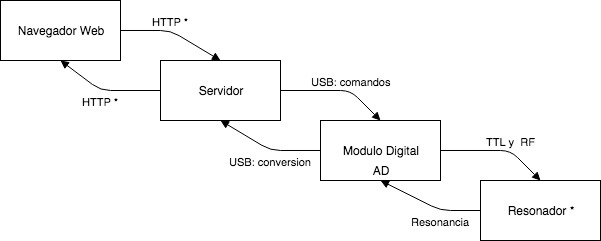
\includegraphics[width=\linewidth]{../figures/d5.jpg}
    \caption{Visi\'on General del sistema}
    \label{fig:d5}
\end{figure}

\subsection{Navegador web}
El navegador web renderiza la \textit{Interfaz Gr\'afica} solicitada al \textit{Servidor}, provee al usuario final 
el control remoto del sistema.

\subsection{Servidor}
El \textit{Servidor} provee servicios REST solicitados por la \textit{Interfaz Gr\'afica} durante la vida
de la sesi\'on del usuario. Estos servicios hacen llamadas al controlador del \textit{M\'odulo
Digital} via USB.

\subsection{M\'odulo Digital}
El \textit{M\'odulo Digital} procesa los mensajes del controlador via USB y ejecuta 
el microc\'odigo del mismo para la configuraci\'on y ejecuci\'on de las secuencias de pulsos.

\subsection{Resonador}
El \textit{Resonador} recibe los pulsos provenientes del \textit{M\'odulo Digital} generando una se\~nal de resonancia
enviada al \textit{M\'odulo Digital} para su conversi\'on digital.

\newpage